\chapter{Einleitung}

In der Software-Entwicklung wird immer mehr Wert auf automatisierte Tests, um die Korrektheit des Programms zu gewährleisten und für die klassische Entwicklung gibt es schon mächtige Werkzeuge, die einen dabei unterstützen. Angefangen mit Test-Frameworks, welche es einem ermöglichen atomare Teile des Codes, bis zu dessen Gesamtheit automatisch zu testen, wodurch man schnelles Feedback erhält und Fehlverhalten leicht aufdecken kann. Darüber hinaus lässt sich mit Code Coverage Analysen feststellen, welche Teile des Codes durch Tests abgedeckt sind. Die Verwendung von Mocking-Frameworks ermöglicht es \textit{Mocks} (\hyperlink{DefinitionMock}{s. Unit-Tests weiter unten}) dynamisch zu erzeugen und deren Verhalten zur Laufzeit zu definieren. Dadurch lassen sich ohne viel Aufwand Teile des Codes komplett isoliert testen. Die testgetriebene Entwicklung stützt sich vollständig auf Tests, indem man zuerst den Test für die neue Funktionalität schreibt, diesen zum Durchlaufen bringen und anschließend refactored. Dadurch erhält man nahezu vollständig durch Tests abgedeckten Code, der offen für Änderungen und robust gegen Fehler ist. Mehr über TDD findet sich in \cite{FRE10}.

Für die Spiele-Entwicklung (mit Unity) gibt es noch keine oder nur sehr einfache Werkzeuge, um seinen Code effektiv zu testen. Deswegen möchte ich in dieser Studienarbeit ein eigenes Framework entwickeln, mit dem sich die verhaltenssteuernden Komponenten eines Spiels testen lassen. Dabei stütze ich mich auf die Erkenntnisse die ich mit einem Kommilitonen in einer vorherigen Studienarbeit \cite{TDGD13} gewonnen habe. Vor allem die Kapitel über die unterschiedlichen \nameref{sec:Testarten}, die Funktionsweise von \nameref{sec:Unity} und wie man aktuell \nameref{chap:Unit Tests mit Unity} mit den vorhandenen Test-Frameworks durchführen kann, sind inhaltlich sehr ähnlich zu der vorangegangenen Arbeit. Dennoch möchte ich diese auf Grund der Nähe zum Thema dieser Arbeit nochmals aufführen.\\
Obwohl es bereits Frameworks für Unity gibt, habe ich mich dazu entschieden von Grund auf ein neues zu entwickeln. Zum einen, um zu erfahren wie schwer es ist ein Test-Framework (für Unity) selbst zu schreiben und zum anderen, um dessen Struktur besser auf meine Bedürfnisse anzupassen.

Im nachfolgenden werde ich zunächst die unterschiedlichen Arten von Tests beschreiben und auf die Funktionsweise von Unity eingehen. Anschließend gebe ich einen Einblick in meine Entwicklungsumgebung.

\section{Testarten}
\label{sec:Testarten}

Tests sollen einen bestimmten Teil des Programms auf seine Korrektheit überprüfen und dabei möglichst schnell und automatisiert ablaufen. Je nachdem wie umfangreich der getestete Bereich ist und welche Kenntnisse der Test/Entwickler von der inneren Umsetzung des Programms hat, kann man diese kategorisieren.

\subsection{White- und Black-Box-Tests}

Die gröbste Einteilung ist die Unterscheidung zwischen White- und Black-Box-Tests. Dabei wird nicht der Umfang des getesteten Bereichs berücksichtigt, sondern lediglich ob der Entwickler des Tests Kenntnisse über die Implementierung der zu testenden Funktionen hat.\\
Bei White-Box-Tests ist dies der Fall. Idealerweise, sollte der Entwickler der den Produktivcode geschrieben hat auch den dazugehörigen Test implementieren. Mit dieser Art von Test werden die inneren Strukturen eines Programms überprüft. Also zum Beispiel, dass eine Methode nicht mit Parametern aufgerufen werden kann, die Fehler verursachen könnten. Hierbei wird nur getestet ob das Programm fehlerfrei abläuft und nicht ob die einzelnen Methoden das gewünschte Verhalten aufweisen.

Im Gegensatz dazu stehen die Black-Box-Tests, deren Entwickler keinerlei Kenntnisse über die Umsetzung haben sollte. Ansonsten könnten beim Schreiben der Tests Dinge implizit als erfüllt angesehen werden, die allerdings getestet werden müssen. Dadurch wäre es möglich, dass bei nachträglichen Änderungen Fehler auftreten, ohne dass ein Test fehlschlägt.\\
Black-Box-Tests sollen verifizieren, dass das Programm die Spezifikationen des Kunden erfüllt.

Diese beiden Testarten ergänzen sich gegenseitig und es sollten immer sowohl White-Box, als auch Black-Box-Tests erstellt werden, um das Produkt zu überprüfen und robust gegen Fehler bei nachträgliche Änderungen zu machen.\\
Schematische Darstellungen dieser Testarten sieht man in \autoref{fig:White_Box_Test} und \autoref{fig:Black_Box_Test} auf der nächsten Seite.

\paragraph{Grey-Box-Tests} stellen eine Mischung aus beiden Varianten dar und vereinen die Eigenschaften beider Arten. Diese erhält man zum Beispiel durch testgetriebene Entwicklung, da man den Test schreibt bevor man den Code implementiert. Dadurch kann man keinerlei Kenntnisse über dessen innere Struktur haben, sondern definiert per Test das erwartete Verhalten. Nachdem dieser erfolgreich ausgeführt wird, erweitert man ihn im Sinne von White-Box-Tests. Dadurch wird sowohl das nach außen sichtbare Verhalten, als auch die innere Struktur des Codes getestet und man benötigt nur einen Entwickler für die Tests.

\clearpage
\begin{figure}[t]
\centering
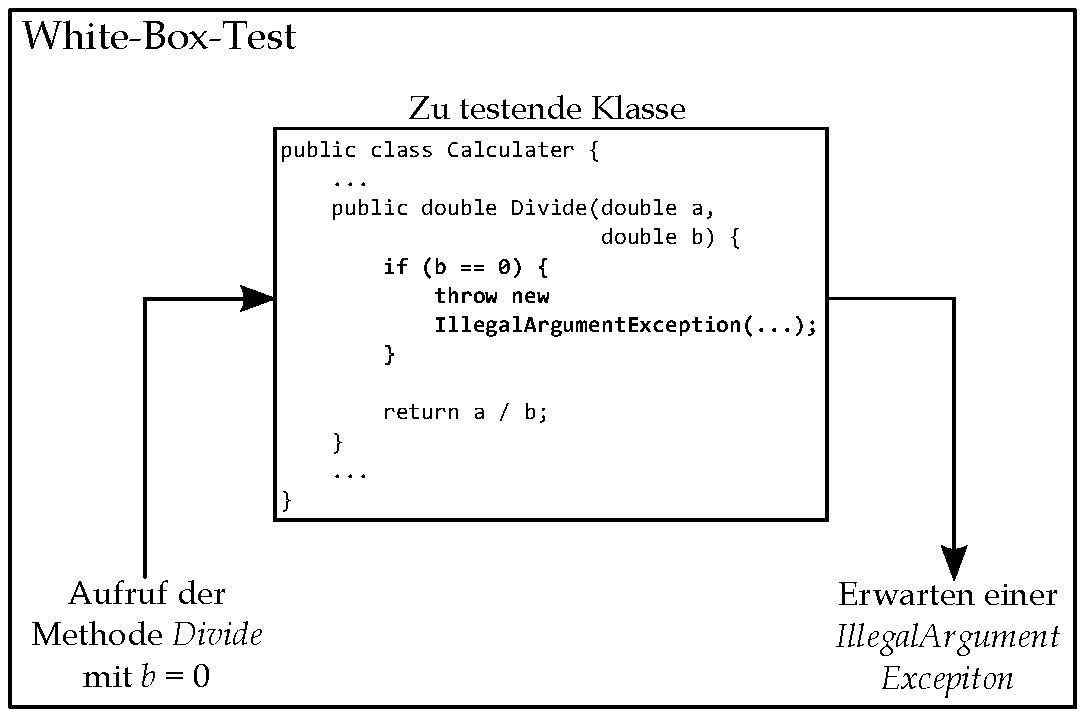
\includegraphics[width=0.8\linewidth]{./images/Kapitel_Einleitung/White_Box_Test.pdf}
\caption[Schematische Darstellung eines White-Box-Tests]{Schematische Darstellung eines White-Box-Tests\\Der Entwickler sollte sich gut mit dem zu testenden Code auskennen. Der Test verifiziert, dass die Methode korrekt ausgeführt wird.}
\label{fig:White_Box_Test}
\end{figure}

\begin{figure}[b]
\centering
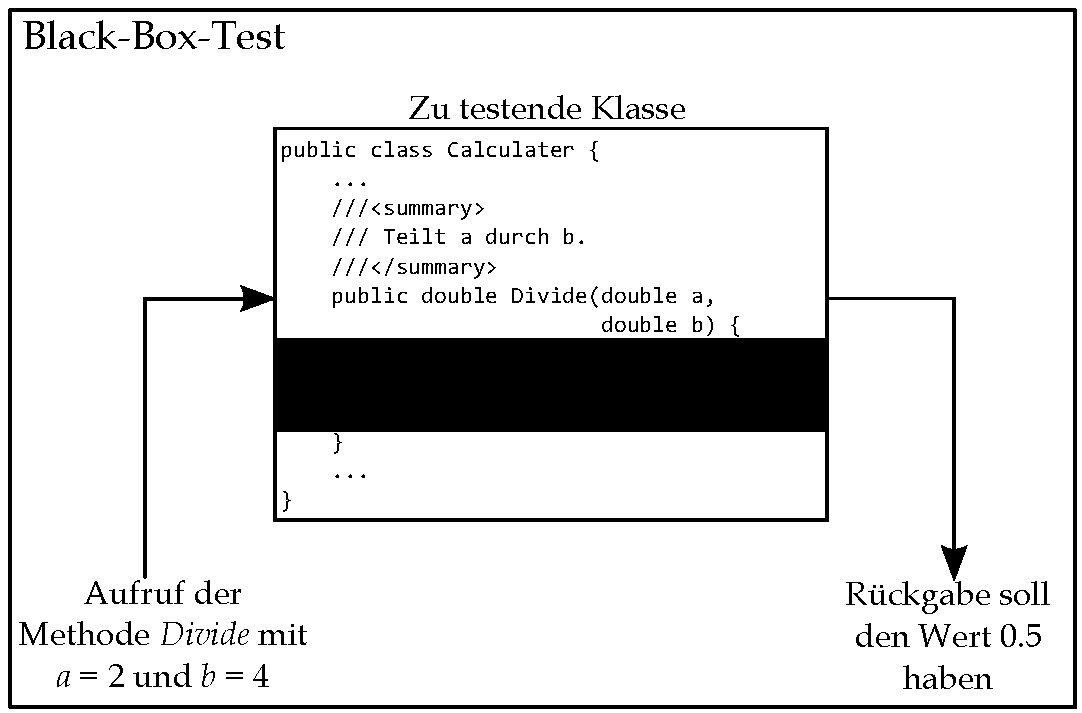
\includegraphics[width=0.8\linewidth]{./images/Kapitel_Einleitung/Black_Box_Test.pdf}
\caption[Schematische Darstellung eines Black-Box-Tests]{Schematische Darstellung eines Black-Box-Tests\\Öffentliche Klassen und Methoden, sowie deren Beschreibungen sind dem Entwickler bekannt. Die konkrete Implementierung allerdings ist nicht einsehbar. Der Test verifiziert das Verhalten der zu testenden Klasse.}
\label{fig:Black_Box_Test}
\end{figure}
\clearpage

\subsection{Unit-Tests} 

Diese sind die kleinsten Einheiten unter den Tests. Sie sollen die einzelnen Methoden einer Klasse auf einen fehlerfreien Ablauf und ein korrektes Verhalten hin testen. Dadurch kann man im Verlauf der Entwicklung Änderungen am Programm vornehmen, ohne dass die Funktionalitäten der Module unbemerkt zerstört werden, insofern die Tests eine ausreichende Abdeckung erreichen (sowohl semantisch, als auch von den Zeilen her).\\
Die einzelnen Tests sollten unabhängig voneinander und auch von den anderen Komponenten sein. Falls Verbindungen zwischen den Komponenten bestehen, sollten diese durch \hypertarget{DefinitionMock}{\textit{Mock}}-Objekte entkoppelt werden. Diese erben von der entsprechenden Klasse und überschreiben deren Methoden auf eine geeignete Art. Zum Beispiel könnten sie einfach leer gelassen werden, was man als \textit{Stub} bezeichnet. Oder sie geben einen festen Wert zurück. \textit{Mock}-Klassen können selbst erstellt werden und sind meistens innere Klassen der Testklasse, allerdings gibt es auch \textit{Mock}-Frameworks, welche generisch \textit{Mocks} für beliebige Klassen oder Interfaces erzeugen können. Das Verhalten der Methoden eines Mocks, lässt sich mit diesen zur Laufzeit festlegen. Zum Beispiel dass ein fester Wert zurückgeliefert wird, oder eine Exception geworfen werden soll.\\ Beispiele sind \textit{JMock} für Java oder \textit{Moq} für C\#.\\
Außerdem sollten Unit-Tests sehr schnell ablaufen (im Millisekunden-Bereich), um nach jeder Änderung durchgeführt werden zu können, ohne die Entwicklung aufzuhalten.

Eine schematische Darstellung von Unit-Tests sieht man in \autoref{fig:Unit_Test}.

\subsection{Integrationstests}

Die nächsthöhere Stufe von Tests sind Integrationstests. Diese testen das Zusammenspiel mehrere Komponenten, eventuell auch mit Systemressourcen, auf ihre Korrektheit. Einen Unit-Test kann man zu einem Integrationstest machen, indem man die \textit{Mock}-Objekte durch die im Produktivbetrieb verwendet Klassen ersetzt und die Bedingungen entsprechend anpasst.

Integrationstests dürfen länger dauern als Unit-Tests, sollten dennoch schnell durchgeführt werden können.

Eine schematische Darstellung von Integrationstests sieht man in \autoref{fig:Integration_Test}.

\subsection{Akzeptanztests} 

Diese sollen die Korrektheit des Verhaltens eines ganzen Systems prüfen. Dabei soll er sowohl die Benutzerschnittstelle, als auch die einzelnen Komponenten und die Systemressourcen abdecken. Allerdings testen diese nicht die innere Struktur des Systems (und sind dementsprechend Black-Box-Tests), sondern sollen gewährleisten, dass ein System sich so verhält, wie es der Kunde im Lastenheft definiert hat. Idealerweise verwendet der Test dabei nur die Schnittstellen, die ein Kunde auch verwenden würde (z.B. über Eingaben auf der GUI), um möglichst nahe an ein natürliches Verhalten zu kommen.\\
Akzeptanztests können durchaus länger dauern, da sie das gesamte Verhalten eines Systems repräsentieren, welches nur nach größeren Veränderungen getestet werden muss.

\begin{figure}[h]
\centering
	\begin{subfigure}[b]{0.29\textwidth}
	\centering
	\captionsetup{justification=centering}
	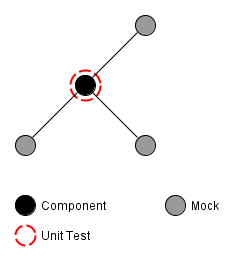
\includegraphics[width=\textwidth]{./images/Kapitel_Einleitung/Unit_Test.png}
	\caption{Unit-Test}
	\label{fig:Unit_Test}
	\end{subfigure}
	\begin{subfigure}[b]{0.29\textwidth}
	\centering
	\captionsetup{justification=centering}
	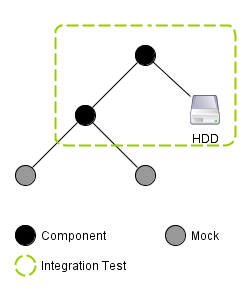
\includegraphics[width=\textwidth]{./images/Kapitel_Einleitung/Integrations_Test.png}
	\caption{Integrationstest}
	\label{fig:Integration_Test}
	\end{subfigure}
	\begin{subfigure}[b]{0.39\textwidth}
	\centering
	\captionsetup{justification=centering}
	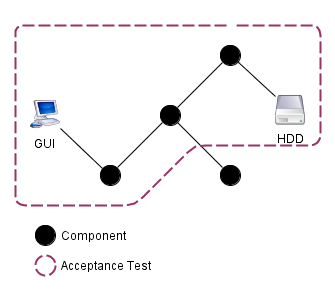
\includegraphics[width=\textwidth]{./images/Kapitel_Einleitung/Akzeptanz_Test.png}
	\caption{Akzeptanztest}
	\label{fig:Acceptance_Test}
	\end{subfigure}
\caption[Schematische Darstellung der unterschiedlichen Testarten]{Schematische Darstellung der unterschiedlichen Testarten\\(a) testet die einzelnen Methoden einer Komponente. Alle anderen benötigten Komponenten sollten als Mock-Objekte eingebunden werden.\\(b) testet das Verhalten mehrere Komponenten und eventuell im Zusammenhang mit Systemressourcen\\(c) testet einen Großteil der Komponenten eines Programms mit den Systemressourcen nach den Anforderungen des Kunden.\\
Quelle: \url{http://schneide.wordpress.com/2011/09/05/a-shot-at-definitions-beyond-unit-test/}}
\label{fig:UnitIntegrationAcceptanceTest_Comparison}
\end{figure}
\clearpage

\section{Unity}
\label{sec:Unity}

\textit{Unity} ist eine Spiele-Engine, welche für viele verschiedene Anwendungen, wie Spiele, Lernsoftware, sowie 3D-Animationsfilme verwendet wird. Der Hersteller bezeichnet die Software selber als \textit{Spieleentwicklungs-Ökosystem}\footnote{Zu lesen unter \url{http://unity3d.com/unity/}}, da sie neben der Engine selber eine komplette Entwicklungsumgebung für Spiele bietet.\\
Die Umgebung erlaubt es einem, die Spiele auch auf andere Plattformen zu portieren, wie zum Beispiel für Android auf Smartphones oder für Webanwendungen. Dies macht die Engine sehr flexibel und ist auch ein Grund für die weite Verbreitung. Der Spielecode für das Spiel lässt sich in verschiedenen Sprachen programmieren, die beim Übersetzen alle von der Unity-Umgebung in die Common Intermediate Language überführt werden, eine Assemblersprache, die erst beim Ausführen in einer Laufzeitumgebung (.NET oder Mono) in nativen Maschinencode übersetzt wird. Die verfügbaren Scriptsprachen sind JavaScript, C\# und Boo\footnote{Weitere Infos zu Boo unter \url{http://boo.codehaus.org/}}.


\paragraph{Unity als Entwicklungsumgebung} Im Mittelpunkt steht ein Szeneneditor, der es ermöglicht die einzelnen Spielszenen zu gestalten, indem die Spielelemente in einem 3D-Editor so angeordnet werden, wie sie im späteren Spiel zu sehen sind. 
Ein Element in einer Szene wird dabei \textit{GameObject} genannt, die Elemente, die zum Einbau bereit stehen, nennt man \textit{Assets}. Ein \textit{Asset} kann dabei vieles sein: Zum Beispiel 3D-Models (\textit{Meshes}), Skripte, Texturen oder Audio-Dateien. \textit{GameObjects} lassen sich beliebig hierarchisch anordnen, um sie so zu gruppieren, oder logisch zu strukturieren. So kann zum Beispiel ein \textit{GameObject} \textit{Spielfigur} die einzelnen Körperteile als Unterobjekte haben, wenn sie als eigene Objekte behandelt werden sollen. Dies vereinfacht zusätzlich den späteren Zugriff auf diese Objekte.\\
Jedem \textit{GameObject} können sogenannte \textit{Components} zugeordnet werden, welche die Eigenschaften und das Verhalten dieses Objektes beschreiben. So muss immer ein \textit{Transform}-Komponente vorhanden sein, das die Position in der Welt, sowie die Rotation und die Skalierung beschreibt. Komponenten können auch Skripte sein, die bei jedem Frame für dieses \textit{GameObject} ausgeführt werden. Es gibt auch Komponenten, die ein \textit{GameObject} zu einem physikalischen Objekt machen, zum Beispiel um ihm eine Gravitationskraft zu geben, oder um Kollisionen zu erkennen. Der Mechanismus zur Kollisionserkennung ist mit Events implementiert. Das heißt, dass in den Skripten eines \textit{GameObjects} zum Beispiel eine \textit{OnCollisionEnter}-Methode vorhanden sein kann, die aufgerufen wird, wenn es mit einem anderen \textit{GameObject} kollidiert. Dies muss nicht unbedingt heißen, dass zwei 3D-Models in der Spielwelt aufeinandertreffen, wenn zum Beispiel ein Projektil einen Gegner trifft. Man kann auch spezielle Kollisions-Boxen für ein Objekt bestimmen, damit zum Beispiel erkannt wird, wenn ein \textit{GameObject} in einen bestimmten Bereich der Spielwelt kommt. Komponenten können auch Texturen, 3D-Modelle, oder Geräuschquellen sein.\\
3D-Modelle können theoretisch auch in einem eigenen 3D-Modellierungstool bearbeitet werden, dies ist allerdings noch nicht ausgereift und wenig komfortabel. Für diese Aufgabe gibt es auch bessere Tools, wie zum Beispiel Blender, welches auch kostenlos verfügbar ist.\\
Mit integriert in die Unity-Umgebung ist Mono-Develop, eine alternative Entwicklungsumgebung für .NET-Sprachen, welche man direkt aus Unity aufrufen kann. Unity bietet die Möglichkeit, das Spiel direkt aus dem Editor übersetzen zu lassen. Dies kann mit einem richtig Build geschehen, allerdings auch für Testzwecke direkt im Editor. Dabei wird aus dem 3D-Viewport einfach die Spieleansicht. Das eignet sich gut für ein schnelles Ausprobieren der Szene, ist allerdings durch eine auf Debugging ausgelegte Kompilierung nicht so schnell, wie der endgültige Build. Am Ende sind die Skripte in einer eigenen .NET-Programmbibliothek vorkompiliert und werden so von der Engine eingebunden.

\paragraph{Unity als Engine} Unity bietet als Spiele-Engine verschiedene Mechanismen, die man bei einem Spiel benötigt. Dies ist in erster Linie eine Grafik-Engine, die die gegebenen Modelle und Texturen in ein Bild auf dem Bildschirm verwandelt. Dazu kommen Engines, die Physikberechnungen durchführen, Audio abspielen, sowie Netzwerkverbindungen für Multiplayer-Spiele bieten.\\
Diese ganzen Engines bilden den Rahmen um das entwickelte Spiel, also die eigenen Skripte, bzw. sonstige eigene Logik. Man muss keine eigene Hauptschleife entwickeln, denn Unity bindet die Skripte ein und führt diese zu entsprechenden Zeitpunkte aus. In jedem Spiel gibt es eine Hauptschleife, die für jeden Frame, der auf dem Monitor angezeigt wird, ausgeführt wird und die Berechnungen durchführt. Dazu wird bei jedem Durchlauf der aktuelle Zustand, sowie Eingaben, wie zum Beispiel Tastendrücke, registriert und daraus der Folgezustand berechnet und auf dem Monitor ausgegeben. Diese Hauptschleife bildet den Kern jedes Spiels.\\
Die Skripte, die nun programmiert werden und das Verhalten der einzelnen Elemente im Spiel beschreiben, müssen von der Unity-Engine interpretierbar sein. Dafür können verschiedene Methoden implementiert werden. \\
Für die folgenden Codebeispiel wurde C\# als Skriptingsprache gewählt, da sie auch unsere verwendete Sprache bei der Entwicklung des Prototypen ist, was später detaillierter betrachtet wird. Bei C\# (und auch bei Boo) gibt es eine Besonderheit, die bei JavaScript nicht beachtet werden muss. Jede Skriptklasse muss hier von \textit{MonoBehaviour} erben. Damit deklariert man diese Klasse als Skript eines \textit{GameObjects} und wird automatisch bei der Engine registriert.\\
Die wichtigste Methode ist \textit{Update()}, welche von der Engine bei jedem Frame aufgerufen wird. Hier müssen alle notwendigen Berechnungen für dieses Objekt und die Änderungen der Spielwelt ausgeführt werden.
Ein sehr einfaches Beispiel für ein Objekt, das sich um die y-Achse drehen soll sieht wie folgt aus.\\

\begin{lstlisting}[caption={[Einfache Skript-Klasse mit Update-Methode]Einfache Skript-Klasse mit Update-Methode}]
using UnityEngine;

public class Beispiel : MonoBehaviour{
	void Update(){
		transform.Rotate(0,5,0);
	}
}
\end{lstlisting}

Die Membervariable \textit{transform} wird von \textit{MonoBehaviour} geerbt und ist eine Referenz auf die zwingend vorhandene \textit{Transform}-Komponente. Diese Komponente lässt sich über verschiedene Methoden beeinflussen, womit man das Objekt drehen, verschieben, oder skalieren kann.\\
Wie man in diesem Beispiel sieht, wird das Objekt bei jedem Frame um den gleichen Winkel gedreht. Dies würde mit einer gleichbleibenden Framerate funktionieren, allerdings kommt das in der Praxis nicht vor. Dafür gibt es in der Engine einen Zeitmechanismus, die Klasse \textit{Time}, die einem Zugriff auf unterschiedliche Zeitinformationen liefert. Dazu gehört \textit{deltaTime}, welche die Zeit in Sekunden beinhaltet, die die Berechnung des letzten Frames gebraucht hat. Damit lässt sich die Methode von oben folgendermaßen schreiben.
\pagebreak

\begin{lstlisting}[caption={[Einfache Update-Methode mit deltaTime]Einfache Update-Methode mit deltaTime}]
	void Update(){
		transform.Rotate(0,5*Time.deltaTime,0);
	}
\end{lstlisting}

Hiermit wird das Objekt nur um 5 Einheiten pro Sekunde verschoben, was die Berechnung unabhängig von der Framerate macht.

Eine weitere wichtige Methode ist \textit{OnGUI()}, in der Dinge implementiert werden, die in der GUI ablaufen sollen. Als GUI bezeichnet man in einem Spiel die Ebene, die über der 3D-Darstellung liegt, wo Menüs, Lebensanzeigen, oder auch Munitions-Stände oder sonstige Status-Elemente platziert werden. \textit{OnGUI} wird bei jedem GUI-Event aufgerufen, wenn zum Beispiel auf ein GUI-Element geklickt wird. Dies kann auch häufiger als der Aufruf von \textit{Update} stattfinden, weshalb diese Aktionen in \textit{OnGUI} verarbeitet werden müssen.

Ein weitere Methode ist \textit{OnCollisionEnter(Collision c)}, welche in einem \textit{GameObject}-Skript aufgerufen wird, wenn ein anderes Objekt in den Kollisionsbereich eintritt. Damit dieser Event-Handler aufgerufen wird, müssen beide Spielobjekte eine sogenannte \textit{Rigidbody}-Komponente haben, welche physikalische Eigenschaften für das Objekt festlegt. Der Methode wird beim Aufruf ein \textit{Collision}-Objekt übergeben, in dem die Daten des kollidierenden Objektes stehen.
\pagebreak

\section{Entwicklungsumgebung}

Wie oben beschrieben, bietet die Unity SDK die Möglichkeit mit mehreren Programmiersprachen zu entwickeln. Um alle Möglichkeiten der objektorientierten Entwicklung nutzen zu können, haben wir uns dazu entschieden den Prototypen in C\# zu schreiben. Dementsprechend nutzen wir neben der Unity SDK noch \textit{Visual Studio 2012} zum programmieren der Logik. Um effizienter entwickeln zu können und aufgrund der besseren Refactoring-Möglichkeiten haben wir \textit{Resharper}\footnote{Für nähere Informationen zu Resharper siehe \url{http://www.jetbrains.com/resharper/}.} installiert. Zusätzlich dazu bietet es einen wesentlich übersichtlicheren Test-Explorer, wie man in der Abbildung auf der nächsten Seite sehen kann.

Zur Verteilung der Aufgaben haben wir Bugzilla\footnote{Für nähere Informationen zu Bugzilla siehe \url{http://www.bugzilla.org/about/}} verwendet. Um die Bugs zu editieren und übersichtlich darzustellen wurde die Lite Version von Deskzilla genutzt.

Damit wir parallel an dem Prototypen arbeiten können, musste das Projekt in einem Git-Repository gespeichert werden, wobei man beim Aufsetzen des Repositories einiges beachten sollte, damit die Verwaltung auch funktioniert. Dies liegt daran, dass manche Dateien in einem Unity-Projekt nur relevant für die SDK des aktuellen Benutzers sind und die Entwicklungsumgebung des Anderen stören würden, falls sie im Repository gespeichert werden. Andererseits befinden sich unter diesen Dateien auch benötigte Information, damit das Projekt korrekt funktioniert, wie zum Beispiel welche Skripte an einem Spielobjekt hängen. Deswegen gibt es die Möglichkeit (seit Version 3.5 auch für die kostenlose Variante von Unity) diese Informationen in Meta-Files abzuspeichern, die sich am selben Ort wie die eigentliche Dateien befinden. Danach muss man noch den Ordner \textit{Library} in das Gitignore-File aufnehmen. Sollte man mehrere Unity-Projekte in einem Repository haben, empfiehlt es sich in jedem Projektordner ein separates Ignore-File anzulegen, um nicht die vollständigen Pfade zu den \textit{Library}-Ordnern angeben zu müssen. Dadurch lassen sich die Ignore-Files für die einzelnen Projekte einfach kopieren.

Eine detaillierte Anleitung zum Verwalten eines Unity-Projekts mit externen Versionierungstools findet man unter \url{http://docs.unity3d.com/Documentation/Manual/ExternalVersionControlSystemSupport.html}.


\begin{figure}[t]
\centering
	\begin{subfigure}[b]{0.45\textwidth}
	\centering
	\captionsetup{justification=centering}
	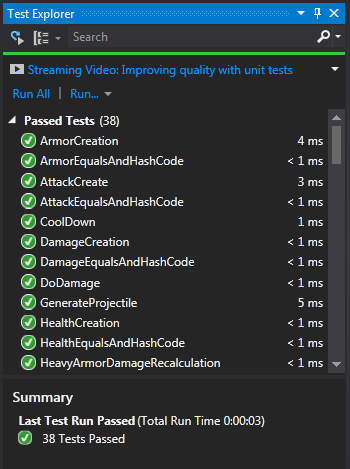
\includegraphics[width=\textwidth]{./images/Kapitel_Einleitung/VisualStudioTestExplorer}
	\caption{Visual Studio 2012}
	\label{fig:VisualStudioTestExplorer}
	\end{subfigure}
	\begin{subfigure}[b]{0.8\textwidth}
	\centering
	\captionsetup{justification=centering}
	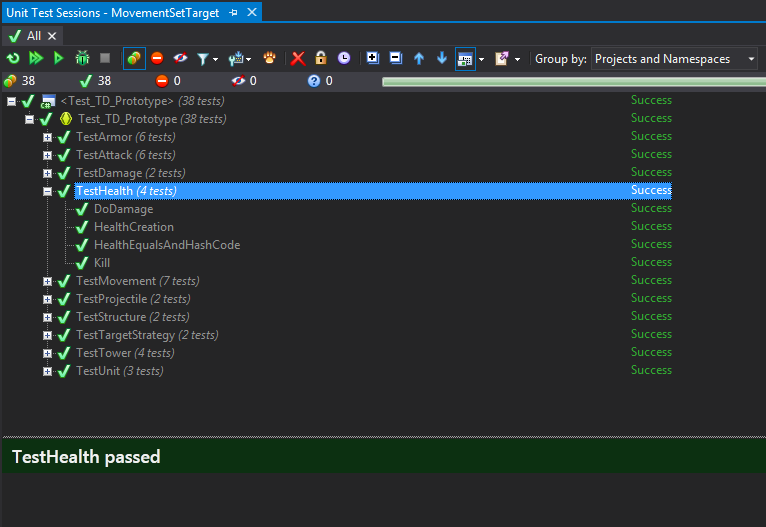
\includegraphics[width=\textwidth]{./images/Kapitel_Einleitung/ResharperTestExplorer}
	\caption{Resharper}
	\label{fig:ResharperTestExplorer}
	\end{subfigure}
\caption[Test Explorer von Visual Studio 2012 und Resharper im Vergleich]{Test Explorer von Visual Studio 2012 und Resharper im Vergleich.}
\label{fig:TestExplorerComparison}
\end{figure}
